\documentclass[12pt]{article}

\usepackage[english]{babel}
\usepackage[utf8x]{inputenc}
\usepackage{amsmath}
\usepackage{graphicx}
\usepackage[colorinlistoftodos]{todonotes}
\usepackage{listings}
\usepackage{glossaries}
\usepackage{placeins}
\usepackage{fixltx2e}
\usepackage{scrpage2}
\usepackage{scrtime}

\clearscrheadfoot
\pagestyle{scrheadings}
\usepackage[
top    = 2.5cm,
bottom = 3cm,
left   = 3cm,
right  = 3cm]{geometry}
\setcounter{secnumdepth}{4}

\author{RoboNav}
\date{\today}


\begin{document}


\begin{titlepage}
\begin{center}
% Oberer Teil der Titelseite:

%NEEDS TO BE OUT COMMENTED sometimes
%\includegraphics[width=1.0\textwidth]{../../pictures/robonavlogo}\\  

\includegraphics[width=0.5\textwidth]{logo}\\  

\LARGE TGM - HTBLuVA Wien XX \\ Ballkomite  \\[1.5cm]

% Title
\rule{1.0\textwidth}{1mm}
{ \huge \bfseries \\[0.4cm]  \huge 2.Ballbesprechung \\ \LARGE HS1 \\[0.4cm] }

\rule{1.0\textwidth}{1mm}



\noindent 
\vspace{6cm}
\small
\begin{center}
  \begin{tabular}{ | p{0.1\textwidth} | p{0.2\textwidth} | p{0.12\textwidth} | p{0.1\textwidth} | p{0.3\textwidth} |}
    \hline
\textbf{Version} & \textbf{Author} & \textbf{Date} & \textbf{Status} & \textbf{Comment} \\ 
    \hline 
    \hline
0.1 & Hannah Siegel & 2014.12.02 & Draft &    \\ 
0.2 & Hannah Siegel & 2014.12.03 & Draft &    \\ 
0.3 & Hannah Siegel & 2014.12.04 & Finished & Ready for Meeting    \\ 

    \hline
  \end{tabular}
\end{center}

\vfill

% Bottom of the page
{\small Version: \today ~at  \thistime    }
\end{center}

%\end{center}
\end{titlepage}
\tableofcontents





%HEADER AND FOOTER
\pagenumbering{arabic}
\ifoot{© Hannah Siegel}
\ofoot{\pagemark }

\section{Anwesenheit}
  \begin{tabular}{ | p{0.3\textwidth} | p{0.1\textwidth} |  p{0.1\textwidth} |}
    \hline
\textbf{Person} & \textbf{1.} & \textbf{2.}  \\ 
    \hline 
    \hline
 
Hannah Siegel & x & \\ \hline
Arian LongHouse & x & \\ \hline
Philipp Vogt & x & \\ \hline
Janusz Gradonski & x & \\ \hline
Daniel Melichar & x & \\ \hline
Dominik Scholz & & \\ \hline
Florian Brandstetter & x & \\ \hline
Nadja Smolnig & x & \\ \hline
Isabella Krammer & x & \\ \hline
Nadja Hauer & x & \\ \hline
Tatjana Gajic & x & \\ \hline
Philip Orosz & x & \\ \hline
Astrid Krickl & & \\ \hline
Richard Bauer & x & \\ \hline
Julia Eichberger & & \\ \hline
Bettina Nedwed & x & \\ \hline
Julia Brandl & x & \\ \hline
Wolfgang Biegel  & x & \\ \hline
Vennesa Belinić & x & \\ \hline
    \hline
  \end{tabular}
\newpage
\section{Hannah traegt vor:}
\subsection{Hardfacts - Wiederholung}
Ball am 21. Februar \\
Einlass 20 Uhr \\
Eroeffnung 21 Uhr\\ \\
TGM und Herbststrasse
\subsection{Besichtigung Palais Auersperg}
Termin muss noch gefunden werden. 
\subsection{DJs}
Diese werden von uns Ausgesucht (ca. 2) \\
Kevin Polley \\
Arian LongHouse  \\
\subsection{Fotografen}
Wird von Herbststrasse geklaert, faellt nciht unter unseren Taetigkeitsbereich.
\subsection{Crash Kurs}
Mittwoch, 28.1.2015 - 14 bis 15 Uhr \\ 
Mittwoch, 04.2.2015 - 14 bis 15 Uhr \\ 
Mittwoch, 11.2.2015 - 14 bis 15 Uhr \\
Donnerstag, 18.2.2015 - 14 bis 15 Uhr \\
\subsection{Eintaenzen}
\subsubsection{Tanzschule}
Tanzschule Elmayer \\
Macht auch Mitternachtseinlage
\subsubsection{Termine der Proben}
Mittwoch, 11.2.2015 - 17 bis 19 Uhr \\ 
Donnerstag, 12.2.2015 - 17 bis 19 Uhr \\
Donnerstag, 19.2.2015 - 17 bis 19 Uhr \\
 \\ \\
Generalprobe am 20.2.2015 im Ballsaal ab 18 Uhr
\subsubsection{Anmeldung zum Eintanzen}
\textbf{Ausnahmslos} ueber Formulare, diese sind auf der naechsten Seite zu finden.
\newpage
\rule{1.0\textwidth}{0.2mm}
\vspace{1cm}
\hspace{1cm}
\textbf{Anmeldung fuer das  Eintanzen des TGM Schulballes 2015} \\
\small
\hspace{3cm}
  \begin{tabular}{ | p{0.4\textwidth} | p{0.5\textwidth}|}
    \hline
\textbf{Name} & \\ 
    \hline 
 \textbf{Geburtsdatum} & \\  \hline 
 \textbf{Schule} & \\  \hline 
 \textbf{Klassenbezeichnung} & \\  \hline 
  \textbf{Email} & \\  \hline 
 \textbf{Telefon} & \\  \hline 

 \textbf{Fixer Partner? } & \\ \hline 
 \textbf{Tanzerfahrung? } & \\
  & \\ \hline 
 \textbf{Schon einmal den TGM Ball eroeffnet (J/N),Anzahl } & \\ \hline 
 \end{tabular}
\vspace{1.5cm}



\rule{1.0\textwidth}{0.2mm}
\vspace{1cm}
\hspace{1cm}
\textbf{Anmeldung fuer das  Eintanzen des TGM Schulballes 2015} \\
\small
\hspace{3cm}
  \begin{tabular}{ | p{0.4\textwidth} | p{0.5\textwidth}|}
    \hline
\textbf{Name} & \\ 
    \hline 
 \textbf{Geburtsdatum} & \\  \hline 
 \textbf{Schule} & \\  \hline 
 \textbf{Klassenbezeichnung} & \\  \hline 
  \textbf{Email} & \\  \hline 
 \textbf{Telefon} & \\  \hline 

 \textbf{Fixer Partner? } & \\ \hline 
 \textbf{Tanzerfahrung? } & \\
  & \\ \hline 
 \textbf{Schon einmal den TGM Ball eroeffnet (J/N),Anzahl } & \\ \hline 
 \end{tabular}
\vspace{0.5cm}
\newpage

\subsection{Plakat}
\begin{figure}[here!]
\centering
\begin{minipage}[h]{0.5\textwidth}
\centering
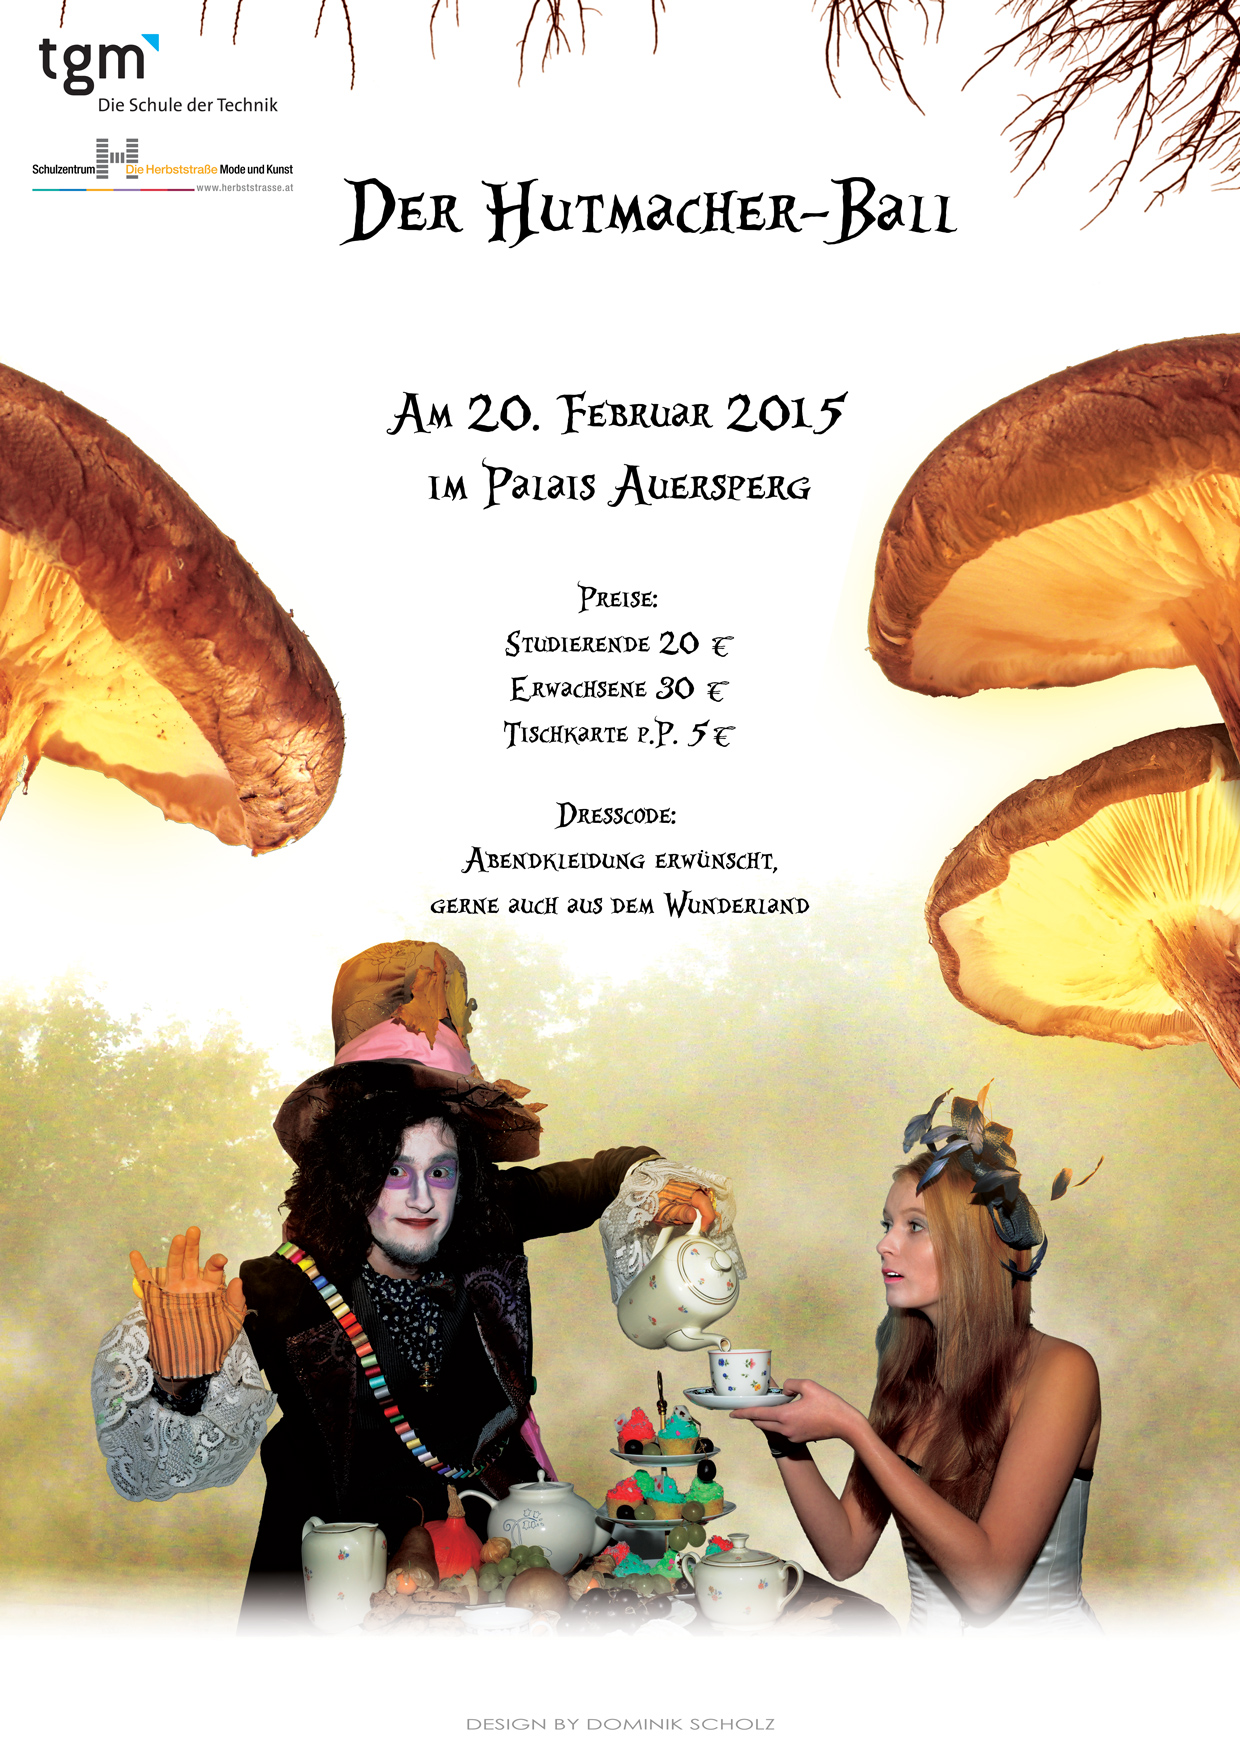
\includegraphics[width=1.0\textwidth]{versionbright_small}
    \caption{Finaler Entwurf}
    \label{fig:eai0}
\end{minipage}
\begin{minipage}[h]{0.45\textwidth}
\centering
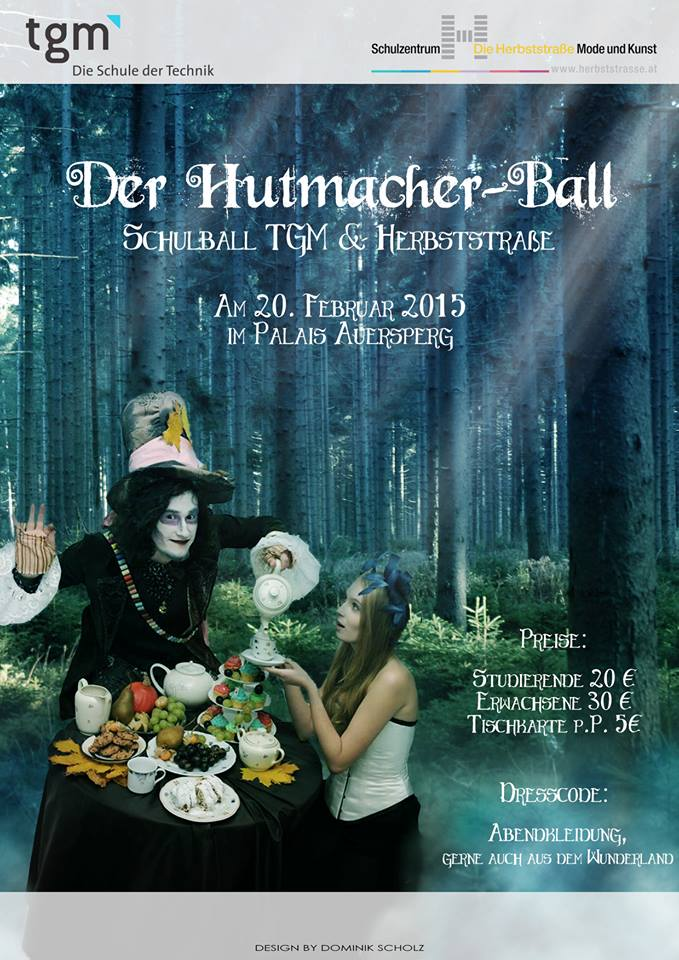
\includegraphics[width=1.0\textwidth]{fertig} 
    \caption{Zweiter Entwurf, gilt nur fuer Herbststrasse}
    \label{fig:eai1}
\end{minipage}
\end{figure}
\newpage
\subsection{Eintrittskarten}
\subsubsection{Kartenverkauf}
Ab \textbf{ 15.Dezember} beim  Verband der TechnologInnen (1.Stock) \\
Eventuell Ausnahmen fuer Abendschueler. \\ \\
Ermaessigt: 20 Euro \\
Normal: 30 Euro
\subsubsection{Gratis Eintritte}
Ihr bekommt, der Regel nach, KEINE Karten.
\begin{enumerate}
\item Eintaenzer gratis Eintritt (Sind frueher da)
\item Schulballkomite gratis (bei Anwesenheit!) (Sind frueher da, stehen auch auf der Liste)
\item Mitternachtseinlagenteilnehmer gratis (betrifft nur Herbststrasse)
\item DJs und Aehnliche gratis (Sind frueher da)
\item AS \& SV vorraussichtlich nicht gratis 
\end{enumerate}
\subsubsection{Tischkarten}
5 Euro pro Person, Verkauf beim Verband der TechnologInnen. \\
Wenn Tische ueber bleiben, bekommt das Ballkomite/die Eintaenzer diese.

\subsection{Deko}
Schach, Poker \\
Stoffe beim Eingang \\
Tischdeko \\
\subsubsection{Technische Deko}
\begin{enumerate}
\item Schulball App
\item Projektpresentation des Apps am Montag vor Weihnachten? Wer will kommen?
\item Polaroid Kameras beim Eingang - Personen werden abgestempelt
\end{enumerate}
\subsection{Ballkoeniging und Ballkoenig}
Wahl vorraussichtlich von dem BESTEN KOSTUEM!
\\
Wahl wahrscheinlich ueber die Schulball-App oder ueber Boxen.
\newpage
\subsection{Organisation am Balltag}
\subsubsection{Meetings}
Es werden fixe Treffpunkte ausgemacht werden (am Balltag und waehrend des Balles)
\subsubsection{Handys}
Jeder sollte sein Handy mithaben bitte.
\subsubsection{Alkohol}
Ist erlaubt, aber wenn ihr Tasks (wie zum Beispiel Kipferl austeilen) habt, bitte \textit{halbwegs} nuechtern :)
\subsubsection{Zeitplan fuer den Balltag}
Ein genauer Zeitplan fuer den Balltag wird beim 3.Ballkomitee treffen presentiert.
\subsubsection{Kontaktinformationen}

 \begin{tabular}{ | p{0.3\textwidth} | p{0.2\textwidth} |  p{0.5\textwidth} |}
    \hline
\textbf{Person} & \textbf{Klasse} & \textbf{Nummer}  \\ 
    \hline 
    \hline
   
Hannah Siegel &  & \\ \hline
Arian LongHouse &  & \\ \hline
Philipp Vogt &  & \\ \hline
Janusz Gradonski&  & \\ \hline
Daniel Melichar&  & \\ \hline
Dominik Scholz &  & \\ \hline
Florian Brandstetter &  & \\ \hline
Nadja Smolnig &  & \\ \hline
Isabella Krammer &  & \\ \hline
Nadja Hauer &  & \\ \hline
Tatjana Gajic &  & \\ \hline
Philip Orosz &  & \\ \hline
Astrid Krickl &  & \\ \hline
Richard Bauer &  & \\ \hline
Julia Eichberger &  & \\ \hline
Bettina Nedwed &  & \\ \hline
Julia Brandl &  & \\ \hline
Wolfgang Biegel  &  & \\ \hline
Vennesa Belinić &  & \\ \hline
  \end{tabular}
\FloatBarrier
\newpage
\section{Input von euch:}
\begin{enumerate}
\item Ideen fuer Verwendung der QR codes?
\item Ideen fuer Umsetzung von Schach und Poker?
\item Brainstorming wegen Hueten der Eintaenzer / Special Dekoration
\item Ideen wegen Aftershow party?
\item Brainstorming wegen Raucherraum
\item hat irgendwer Wakey Talkies zuhause?
\item \textbf{ANDERE IDEEN}? - Am ende :)
\end{enumerate}

\newpage
\section{Einteilung}
  \begin{tabular}{ | p{0.35\textwidth} | p{0.20\textwidth} |  p{0.5\textwidth} |}
    \hline
\textbf{Aufgabe} & \textbf{Datum / Uhrzeit} & \textbf{Personen / Veranntwortlichen} \\ 
    \hline 
    \hline
\textbf{Vorm Balltag} &  &  \\ 
  &  &  \\ \hline
DJs auswaehlen (4) & bis ende Dezember &  \\ 
  &  &  \\ \hline
Organisation After show Party wenn gewollt (2) & bis Anfang Jaenner &  \\ \hline
Organisation Crashkurs (1) & bis mitte Dezember &  \\ \hline
\textit{Organisation Wahl des besten Kostuemes (2)} & bis mitte Jaenner &  \\ \hline
\textbf{Am Balltag} &  &  \\ 
  &  &  \\ \hline
Kipferl holen (2) & ca 14:00 & Bettina Nedwed \& Isabella Krammer \\ \hline
Kipferl einpacken (4) & ca 15:00 &\\ 
  &  &  \\ \hline
Kipferl austeilen Schicht 1 (2) & von 0:30 bis 1:30 &   \\ \hline
Kipferl austeilen Schicht 2 (2) & von 1:30 bis ende &   \\ \hline
Karten abreissen Schicht 1 (2) & von Anfang bis 22:00 &   \\ \hline
Karten abreissen Schicht 2 (2) & von 22:00 bis noetig &   \\ \hline
Deko helfen (4) & Ganzen Nachmittag &  \\
  &  &  \\ \hline
DJs Aufbauen helfen (1) & ca 19:00 &  \\ \hline
Beim Fotografen aufbauen helfen (2) & ca 17:00 &  \\ \hline
Eintaenzer organisieren (1) &  ca 18:00 &  \\ \hline
Mitternachtseinlage helfen (1) & ca 22:00 &  \\ \hline
\textit{Auszaehlen Wahl des besten Kostuemes (6)} & kurz vor 24:00 &  \\ 
  &  &  \\ 
  &  &  \\ \hline
\textbf{ALLE} &  &  \\ 
  &  &  \\ \hline
Vorm Eintanzen den Ballsaal fuellen, platz machen &  & Alle  \\ \hline
Durchgehen und kontrollieren ob alles passt &  & Alle  \\ \hline
Durch die Klassen gehen und die Informationen verteilen & bis 15. Dezember &  Alle\\ \hline
Plakate aufhaengen & mitte Dezember & Alle  \\ \hline

\hline
\end{tabular}
  
%Arian LongHouse 
%Philipp Vogt 
%Janusz Gradonski
%Daniel Melichar 
%Dominik Scholz
%Florian Brandstetter 
%Nadja Smolnig
%Isabella Krammer 
%Nadja Hauer 
%Tatjana Gajic 
%Philip Orosz
%Astrid Krickl 
%Richard Bauer 
%Julia Eichberger
%Bettina Nedwed
%Julia Brandl 
%Vennesa Belinić 
%Wolfgang Biegel
\subsection{Verantwortliche / Chefes}

\begin{tabular}{ | p{0.4\textwidth} | p{0.6\textwidth}  |}
    \hline
\textbf{Aufgabe} & \textbf{Verantwortlicher (VORSCHLAG!)}  \\ 
    \hline 
    \hline
  
DJs  & Arian LongHouse \& \\ \hline
Erste Hilfe & Hannah Siegel \& \\ \hline
Securities  & Hannah Siegel \& \\ \hline
Eintaenzer & Isabella Krammer \& \\ \hline
Ballkomite &  Hannah Siegel \& \\ \hline
Probleme &  Hannah Siegel \& \\ \hline
  \end{tabular}

\subsection{Klasseneinteilung}
  \begin{tabular}{ | p{0.4\textwidth} | p{0.3\textwidth} |  p{0.3\textwidth}  |}
    \hline
\textbf{Person} & \textbf{Abteilung} & \textbf{Jahrgaenge} \\ 
    \hline 
    \hline
 
Philipp Vogt & KT & 1,2,3,4,5 \\ \hline
Janusz Gradonski & IT &  1,2,3,4 \\ \hline
Daniel Melichar & IT & 1,2,3,4 \\ \hline
Florian Brandstetter & BM & 1,2 \\ \hline
Nadja Smolnig & WI & 1,2,3,4,5 \\ \hline
Isabella Krammer & BM & 1,2  \\ \hline
Nadja Hauer & BM & 3  \\ \hline
Tatjana Gajic & EL & 1,2,3,4,5 \\ \hline
Philip Orosz & IT &  1,2,3,4 \\ \hline
Astrid Krickl & IT & 5 \\ \hline
Richard Bauer & ET & 1,2,3,4,5 \\ \hline
Julia Eichberger & MI & 1,2,3,4,5\\ \hline
Wolfgang Biegel  & AS? & \\ \hline
  \end{tabular}
  \subsection{Naechste Treffen}
  Wenn nicht anders Angegeben, dann in der Aula des 9. Stocks :) \\
  Andere kleinere (noetige) Besprechungen werden einfach spontan ausgemacht. \\
 \begin{tabular}{ | p{0.3\textwidth} | p{0.2\textwidth} |  p{0.5\textwidth} |}
    \hline
\textbf{Treffen} & \textbf{Termin} & \textbf{Personen}  \\ 
    \hline 
    \hline

DJs & 9.1 - 9:50 & mit DJs \\ \hline
After Show Party & 22.12 - 9:50 &  \\ \hline
After Show Party & 8.1 - 9:50 &  \\ \hline
After Show Party & 2.2 - 9:50 &  \\ \hline
Crashkurs & 16.12 - 9:50 &  \\ \hline
Austeilung Plakate & 12.12 - 9:50 & alle \\ \hline
Kipferl  & 20.02 - 9:50 &  \\ \hline
Karten  & 19.02 - 9:50 &  \\ \hline
SchulballApp  & 22.12 - ca 6.Stunde &  \\ \hline
'BallkoenigIn'  & 22.12 - 9:50 &  \\ \hline
'BallkoenigIn'   & 28.01 - 9:50 &  \\ \hline
\textbf{3 . Ballkomite treffen}   & 25.01 - 11.Stunde & alle - wsl HS1 \\ \hline
\textbf{4 . Ballkomite treffen}   & 12.02 - 11.Stunde & alle - wsl HS1 \\ \hline
\textbf{Balltag}  & \textbf{21.02 - 19:00} & \textbf{alle} \\ \hline


  \end{tabular}
  \newpage

\end{document}
